\documentclass[apj, revtex4]{emulateapj}

\usepackage{epsf}
\usepackage{color}
\usepackage{amsmath}
\usepackage{graphicx}
\usepackage[colorlinks,urlcolor=blue,citecolor=blue,linkcolor=blue]{hyperref}
\usepackage{threeparttable}
\usepackage{multirow}
\usepackage{natbib}
\usepackage{etoolbox}

\bibliographystyle{apj}
\citestyle{aa}
 
% General commands that are good for any astronomy paper.
%%% Fields %%%
\newcommand{\hdf}{HDF-N}
\newcommand{\hdfn}{HDF-N}
\newcommand{\hdfs}{HDF-S}
\newcommand{\cdfs}{CDF-S}

%%% Telescopes %%%
\newcommand{\hst}{\textit{HST}}
\newcommand{\iras}{\textit{IRAS}}
\newcommand{\iso}{\textit{ISO}}
\newcommand{\spitzer}{\textit{Spitzer}}
\newcommand{\sirtf}{\textit{Spitzer}}
\newcommand{\chandra}{\textit{Chandra}}

%%% Filters %%%
\newcommand{\wfu}{\hbox{$\mathrm{U}_{300}$}}
\newcommand{\wfb}{\hbox{$\mathrm{B}_{450}$}}
\newcommand{\wfv}{\hbox{$\mathrm{V}_{606}$}}
\newcommand{\wfi}{\hbox{$\mathrm{I}_{814}$}}
\newcommand{\acsb}{\hbox{$\mathrm{B}_{435}$}}
\newcommand{\acsv}{\hbox{$\mathrm{V}_{606}$}}
\newcommand{\acsi}{\hbox{$i_{775}$}}
\newcommand{\acsz}{\hbox{$z_{850}$}}
\newcommand{\nicj}{\hbox{$\mathrm{J}_{110}$}}
\newcommand{\nich}{\hbox{$\mathrm{H}_{160}$}}
\newcommand{\wfcy}{\hbox{$\mathrm{Y}_{105}$}}
\newcommand{\wfcj}{\hbox{$\mathrm{J}_{125}$}}
%\newcommand{\wfcj}{\hbox{$J_{110}$}}
\newcommand{\wfch}{\hbox{$\mathrm{H}_{160}$}}
\newcommand{\sdssu}{\hbox{$u$}}
\newcommand{\sdssg}{\hbox{$g$}}
\newcommand{\sdssr}{\hbox{$r$}}
\newcommand{\sdssi}{\hbox{$i$}}
\newcommand{\sdssz}{\hbox{$z$}}
\newcommand{\mone}{\hbox{$[3.6]$}}
\newcommand{\mtwo}{\hbox{$[4.5]$}}
\newcommand{\mthree}{\hbox{$[5.8]$}}
\newcommand{\mfour}{\hbox{$[8.0]$}}
%\newcommand{\mone}{\hbox{$[3.6\mu\mathrm{m}]$}}
%\newcommand{\mtwo}{\hbox{$[4.5\mu\mathrm{m}]$}}
%\newcommand{\mthree}{\hbox{$[5.8\mu\mathrm{m}]$}}
%\newcommand{\mfour}{\hbox{$[8.0\mu\mathrm{m}]$}}

%%% Astronomy Abreviations %%%
\newcommand{\mstar}{\hbox{$\mathrm{M}^\ast$}}
\newcommand{\lstar}{\hbox{$L^\ast$}}
\newcommand{\Msol}{\hbox{$\mathrm{M}_\odot$}}
\newcommand{\msol}{\hbox{$\mathrm{M}_\odot$}}
\newcommand{\Zsol}{\hbox{$Z_\odot$}}
\newcommand{\zsol}{\hbox{$Z_\odot$}}
\newcommand{\Lsol}{\hbox{$L_\odot$}}
\newcommand{\lsol}{\hbox{$L_\odot$}}
\newcommand{\lir}{\hbox{$L_{\mathrm{IR}}$}}
\newcommand{\zph}{\hbox{$z_\mathrm{ph}$}}
\newcommand{\zphot}{\hbox{$z_\mathrm{ph}$}}
\newcommand{\lbol}{\hbox{$L_\mathrm{bol}$}}
\newcommand{\snr}{\hbox{$\mathrm{S/N}$}}
\newcommand{\reff}{\hbox{$r_\mathrm{eff}$}}
\newcommand{\ks}{\hbox{$K_s$}}
\newcommand{\AAA}{\hbox{\AA}}

%%% Spectrum Lines %%%
\newcommand{\lya}{ Ly$\alpha \;$}
\newcommand{\lyb}{Lyman~$\beta$}
\newcommand{\hb}{\hbox{H$\beta$}}
\newcommand{\ha}{\hbox{H$\alpha$}}
\newcommand{\paa}{\hbox{Pa$\alpha$}}

%%% Units %%%
\newcommand{\kms}{\hbox{km~s$^{-1}$}}
\newcommand{\cms}{\hbox{cm~s$^{-1}$}}
\newcommand{\mpc}{\hbox{Mpc$^{-1}$}}
\newcommand{\mpcsq}{\hbox{Mpc$^{-2}$}}
\newcommand{\mpccu}{\hbox{Mpc$^{-3}$}}
\newcommand{\cnts}{\hbox{cnt~s$^{-1}$}} 
\newcommand{\cmsq}{\hbox{cm$^{-2}$}}
\newcommand{\cmcu}{\hbox{cm$^{-3}$}}
\newcommand{\ergscm}{\hbox{erg~s$^{-1}$~cm$^{-2}$}}
\newcommand{\uJy}{\hbox{$\mu$Jy}}
\newcommand{\ujy}{\hbox{$\mu$Jy}}
\newcommand{\degree}{\hbox{$^\circ$}}
\newcommand{\degsq}{\hbox{degree$^2$}}
\newcommand{\arcminsq}{\hbox{arcmin$^2$}}
\newcommand{\um}{\hbox{$\mu$m}}

%%% Math %%%
\newcommand{\lsim}{\lesssim}
\newcommand{\gsim}{\gtrsim}
\newcommand{\mathS}{\hbox{$\mathcal{S}$}}
\newcommand{\mathR}{\hbox{$\mathcal{R}$}}
\newcommand{\mathM}{\hbox{$\mathcal{M}$}}
\newcommand{\mcal}{\hbox{$\mathcal{M}$}}
\newcommand{\rcal}{\hbox{$\mathcal{R}$}}
\newcommand{\scal}{\hbox{$\mathcal{S}$}}
\newcommand{\infinity}{\hbox{$\infty$}}
\newcommand{\err}[2]{$^{+#2}_{-#1}$}

%%% General %%%
\newcommand{\etal}{et al.}
\newcommand{\eg}{e.g.}
\newcommand{\ie}{i.e.}
\newcommand{\cf}{cf.}
% \newcommand{\ion}[2]{\hbox{#1$\;${\small\rm{#2}}}}
\newcommand{\mybullet}{\noindent$\bullet$}
\newcommand{\uit}{\textit{UIT}}
\newcommand{\nd}{...}
%\newcommand{\cmodel}{\hbox{\tt cmodel}}
%\newcommand{\bs}{\hbox{$\!\!\!\!$}}
\newcommand{\todo}[1]{{\tt #1}}
\newcommand{\citeeg}[1]{(\eg, \citealt{#1})}
\newcommand{\ignore}[1]{}

%%% Extra %%% 
% \newcommand{\farcm}{\mbox{\ensuremath{.\mkern-4mu^\prime}}}%fractional arcminute symbol 0.'0
% \newcommand{\farcs}{\mbox{\ensuremath{.\!\!^{\prime\prime}}}}%fractional arcsecond symbol: 0.''0
% \newcommand{\fdg}{\mbox{\ensuremath{.\!\!^\circ}}}%fractional degree symbol:     0.°0
\newcommand{\arcdeg}{\ensuremath{^{\circ}}}%                    % degree symbol:  °
% \newcommand{\sun}{\ensuremath{\odot}}%                          % sun symbol
% \newcommand{\apj}{ApJ}%                                         % Journal abbreviations
% \newcommand{\apjs}{ApJS}
% \newcommand{\apjl}{ApJL}
% \newcommand{\aap}{A{\&}A}
% \newcommand{\aaps}{A{\&}AS}
% \newcommand{\mnras}{MNRAS}
% \newcommand{\aj}{AJ}
% \newcommand{\araa}{ARAA}
% \newcommand{\pasp}{PASP}
\newcommand{\Teff}{\ensuremath{T_{\mathrm{eff}}}}%              % T_eff
\newcommand{\logg}{\ensuremath{\log g}}%                        % log g
\newcommand{\bv}{\ensuremath{B\!-\!V}}%                         % B-V
\newcommand{\ub}{\ensuremath{U\!-\!B}}%                         % U-B
\newcommand{\vr}{\ensuremath{V\!-\!R}}%                         % V-R
\newcommand{\ur}{\ensuremath{U\!-\!R}}%                         % U-R

\makeatletter
% Patch case where name and year are separated by aysep
\patchcmd{\NAT@citex}
  {\@citea\NAT@hyper@{%
     \NAT@nmfmt{\NAT@nm}%
     \hyper@natlinkbreak{\NAT@aysep\NAT@spacechar}{\@citeb\@extra@b@citeb}%
     \NAT@date}}
  {\@citea\NAT@nmfmt{\NAT@nm}%
   \NAT@aysep\NAT@spacechar\NAT@hyper@{\NAT@date}}{}{}

% Patch case where name and year are separated by opening bracket
\patchcmd{\NAT@citex}
  {\@citea\NAT@hyper@{%
     \NAT@nmfmt{\NAT@nm}%
     \hyper@natlinkbreak{\NAT@spacechar\NAT@@open\if*#1*\else#1\NAT@spacechar\fi}%
       {\@citeb\@extra@b@citeb}%
     \NAT@date}}
  {\@citea\NAT@nmfmt{\NAT@nm}%
   \NAT@spacechar\NAT@@open\if*#1*\else#1\NAT@spacechar\fi\NAT@hyper@{\NAT@date}}


%Commands specific to the this work
\newcommand{\editorial}[1]{\textcolor{red}{#1}}
\DeclareRobustCommand{\ion}[2]{%
\relax\ifmmode
\ifx\testbx\f@series
{\mathbf{#1\,\mathsc{#2}}}\else
{\mathrm{#1\,\mathsc{#2}}}\fi
\else\textup{#1\,{\mdseries\textsc{#2}}}%
\fi}

%-----------------------------------------------------------------------------------------

\shorttitle{Cluster Dynamics with HETDEX}
\shortauthors{BOADA ET AL.}

%\slugcomment{\it Draft Version \today}
%\slugcomment{\it Submitted for publication in the Astrophysical Journal}
%\slugcomment{Accepted for Publication in the Astrophysical Journal}

\begin{document}

\title{Cluster Dynamics with HETDEX - I: Simulated Performance, Mass Distribution and Limits}

\author{\sc Steven Boada\altaffilmark{1}, 
C.~Papovich\altaffilmark{1}, and
R.~Wechsler\altaffilmark{2,3}} 

\altaffiltext{1}{George P.\ and Cynthia Woods Mitchell Institute for
Fundamental Physics and Astronomy, and Department of Physics and Astronomy,
Texas A\&M University, College Station, TX, 77843-4242;
boada@physics.tamu.edu}
\altaffiltext{2}{Kavli Institute for Particle Astrophysics and Cosmology, Department of Physics, Stanford University, Stanford, CA 94305, USA}
\altaffiltext{3}{Department of Particle Physics and Astrophysics, SLAC National Accelerator Laboratory, Menlo Park, CA 94025, USA}

\begin{abstract}
\noindent
ABSTRACT GOES HERE!!
Lorem ipsum dolor sit amet, consectetur adipisicing elit, sed do eiusmod tempor incididunt ut labore et dolore magna aliqua. Ut enim ad minim veniam, quis nostrud exercitation ullamco laboris nisi ut aliquip ex ea commodo consequat. Duis aute irure dolor in reprehenderit in voluptate velit esse cillum dolore eu fugiat nulla pariatur. Excepteur sint occaecat cupidatat non proident, sunt in culpa qui officia deserunt mollit anim id est laborum.
\end{abstract}

\section{INTRODUCTION}
Our ability to perform precision cosmology with clusters of galaxies has reached a critical turning point. The widely accepted $\Lambda$CDM model of cosmology makes explicit predictions about the number and masses of galaxy clusters throughout the universe. However, connecting these predictions to a set of, sufficiently large in size, observed clusters remains a principal problem. Specifically, the largest threat to modern, precision, cluster cosmology is not the identification of large numbers of clusters (the total number of clusters known is only going up) but the accurate recovery of galaxy cluster mass \citeeg{Sehgal2011,Plank2014, Bocquet2015}.

As mass is not a direct observable, a lot of work is underway to characterize galaxy cluster masses with an observable feature of galaxy clusters. The goal is to constrain, as best possible, $P(X|M,z)$ the probability ($P$) that a galaxy cluster of given mass ($M$), located at redshift ($z$) determined using observable parameter ($X$). The observable parameter most commonly observed X-ray temperatures and luminosities \citeeg{Mantz2010, Rykoff2014, Mantz2015}, cosmic microwave background observations \citeeg{Vanderlinde2010, Sehgal2011} using the Sunyaev--Zel’dovich effect (SZE; \citealt{Sunyaev1972}) or optical studies \citeeg{Rozo2010, Rozo2014} of richness \citeeg{Abell1958,Rykoff2012} or galaxy velocity dispersions \citeeg{Ruel2014, Sifon2015}.

Massive surveys, both on going and planned, are revolutionizing cluster cosmology using a large range of wavelengths. The South Pole Telescope (SPT; \citealt{Carlstrom2011}) and the Atacama Cosmology Telescope (ACT; \citealt{Swetz2011}) are discovering many clusters through the SZE. Optically, the on going The Dark Energy Survey (DES; \citealt{DES2005}) and planned Large Synoptic Survey Telescope (LSST; \citealt{LSST2012}) will identify many thousands of clusters to much lower masses than is possible with SZE measurements. However, regardless of the discovery method used, spectroscopic followup is needed to further constrain $P(X|M,z)$. But as the cluster dataset grows to many tens of thousands of clusters individual followup becomes increasingly impractical. Therefore, large spectroscopic surveys are needed to more fully constrain the observable--mass relation of clusters.

The Hobby Eberly Telescope Dark Energy eXperiment (HETDEX; \citealt{Hill2008}) is a trailblazing effort to observe high-redshift large scale structures using cutting edge wide-field integral field unit (IFU) spectrographs. Designed to probe the evolution of the dark energy equation of state etched onto high redshift ($z>2$) galaxies by the Baryon Acoustic Oscillations \citep{Eisenstein2005} in the first moments of the universe, the survey will observe two fields for a total of 420 \degsq\ from two fields (300 \degsq, Spring field and 120 \degsq, Fall field). Tuned to find \lya\ emitting (LAE) galaxies at $1.9<z<3.5$, HETDEX expects to find 800,000 LAEs, and more than one million [\ion{O}{ii}] emitting galaxies at $z<0.5$ masquerading as high-redshift galaxies \citep{Acquaviva2014}.  

While a large portion of the $\sim10^6$ interloping [\ion{O}{ii}] galaxies will be field (not associated with a bound structure) galaxies, the large area covered by HETDEX is expected to contain as many as 100 Virgo-sized ($M_{dyn}\sim 10^{15}$ \msol) clusters at $z<0.5$ (\editorial{citation?}). The near-complete spectroscopic coverage allows an unprecedentedly detailed look at a very large number of clusters ranging from group scales to the very massive. In addition to the recovery of accurate dynamical masses, detailed investigations of the of dynamical state of the clusters is possible. 

Connecting the dynamical properties derived from spectroscopy to the properties inferred from other studies insures the greatest impact on future work. HETDEX overlaps with the Sloan Digital Sky Survey (SDSS; \citealt{Blanton2001a}), SDSS stripe 82 \citep{Annis2014}, the Dark Energy Survey (DES; \citealt{DES2005}), and the upcoming DECam/IRAC Galaxy Environment Survey (DIRGES; PI: Papovich, C. Papovich \etal\ in preparation). \editorial{SHELA and others? Would be good to have a whole list of different things and different wavelengths.} While the potential dataset is very rich, two large issues remain.

It is unclear how a blind spectroscopic survey with an IFU will effect the recovery of galaxy cluster dynamical properties. Unlike many previous large cluster surveys \citeeg{Milvang-Jensen2008, Robotham2011, Sifon2015} which use multi-object spectrographs, the Visible Integral-Field Replicable Unit Spectrograph (VIRUS; \citealt{Hill2012}) used by HETDEX samples the sky unevenly which could excluded member galaxies which would otherwise be included. Secondly, it is not straightforward to use spectroscopic redshifts predominately from emission-line galaxies to interpret the kinematic and dynamical states of the clusters.

This work plans to address these concerns in the following ways. We use simulated observations which target individual galaxy clusters to investigate the recovery of parameters with such observations. Secondly, we create and evaluate a HETDEX like selection ``function'' of galaxies over a similarly large portion of the sky and use well adopted techniques to recover the dynamical properties, such as velocity dispersion and mass. Each observation strategy will further be constrained with ``ideal'' and ``realistic'' knowledge. Ideal knowledge assumes that we know which individual galaxy is assigned to which cluster. With realistic knowledge this is unknown and must be determined prior to the estimation of the cluster properties. Both of these strategies will better allow future work to predict the number and types of galaxy clusters which should be observed with VIRUS during both the HETDEX survey portion and through targeted follow up observations.

\editorial{Give outline of paper section.}

Throughout this paper, we adopt the following cosmological model ($\Omega_\Lambda = 0.77$,
$\Omega_M = 0.23$, $\sigma_8 = 0.83$ and $H_0= 72$ \kms \mpc), assume a Chabrier initial mass function (IMF; \citealt{Chabrier2003}), and use AB magnitudes \citep{Oke1974}.

\section{Data and Mock Observations}\label{sec:Data}

Blah blah intro stuff... 

\subsection{The ``Buzzard'' Catalogs}
The ``Buzzard'' mock galaxy catalogs (R. Wechsler et al., private communication) are derived from a combination of Sub-halo Abundance Matching (ShAM) and ADDSEDs (Adding Density Dependent Spectral Energy Distributions) tied to an in house n-body cosmological simulation. A brief description of the catalog creation is described as follows. The initial conditions are generated with a second-order Lagrangian perturbation theory using {\tt 2LPTic} \citep{Crocce2006}. Dark matter (DM) n-body simulations are run using {\tt LGadget-2} (a version of {\tt Gadget-2}; \citealt{Springel2005}). The DM halos are identified using the {\tt ROCKSTAR} halo finder \citep{Behroozi2013} which also calculates halo masses and other various parameters. 

Galaxy $M_r$ luminosities are added to the velocity peaks using ShAM \citep{Reddick2013}, and ADDSEDs (Adding Density Dependent Spectral Energy Distributions) assign luminosities in the other bands. A $M_r$-density-SED relation is created using a SDSS training set, and for each mock galaxy the SED of a randomly selected training set galaxy which has a similar $M_r$ and density is assigned. The result is a 398.49 sq. degree mock catalog occupying a $60 \leq RA \leq 90$ and $-40 \leq DEC \leq -61$ portion of the sky. It contains 238 million galaxies with \sdssr\ mag $< 29$ and $z \leq 8.7$.

The catalog information, used in this study, is broken into two large portions. The ``truth'' files contain the characteristics of each individual galaxies, such as right ascension (RA), declination (DEC), redshift (z), observed and rest-frame magnitudes, and many others. The ``halo'' files contain information for individual halos, to which many individual galaxies may belong. This includes five estimations of dynamical mass, RA, DEC, z, three dimensional velocity dispersion, and many others.

However, the catalogs do not include information on emission or absorption lines or estimations of whether the halo is relaxed or not. We supplement the catalogs with this information and describe the method in Section~\ref{sec:oii luminosity} and others.

\begin{figure} 
	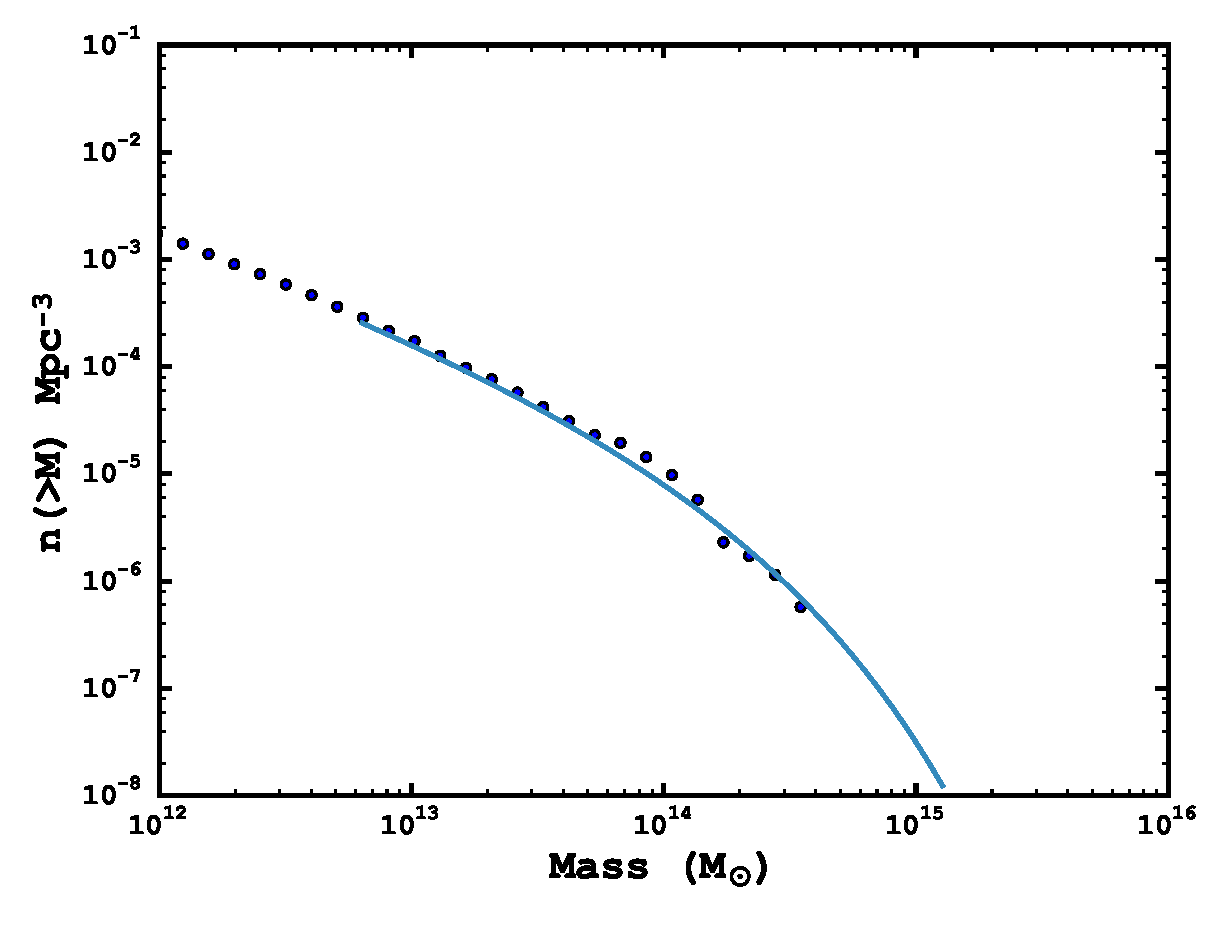
\includegraphics[width=0.49\textwidth]{hmf.pdf} 
	\caption{The cumulative MF of halos above $M_{200c}$ at $z=0.1$. The predicted MF is from \cite{Tinker2008}.} 
	\label{fig:hmf} 
\end{figure}

We investigate the accuracy of the halo mass distribution by comparing the cumulative number density of halos above a mass ($M_{200c}$) threshold to the halo mass function (HMF) of \cite{Tinker2008}. Shown in Figure~\ref{fig:hmf} the HMF is calculated at central redshifts of 0, 0.2, and 0.4 using {\tt HMFcalc} \citep{Murray2013} and compared to galaxies in a redshift window of $\Delta z\pm0.01$. We find a very good agreement between the expected HMF and the observed. 

\subsection{ {\rm[\ion{O}{ii}]} Luminosity}\label{sec:oii luminosity}
\begin{figure*} 
	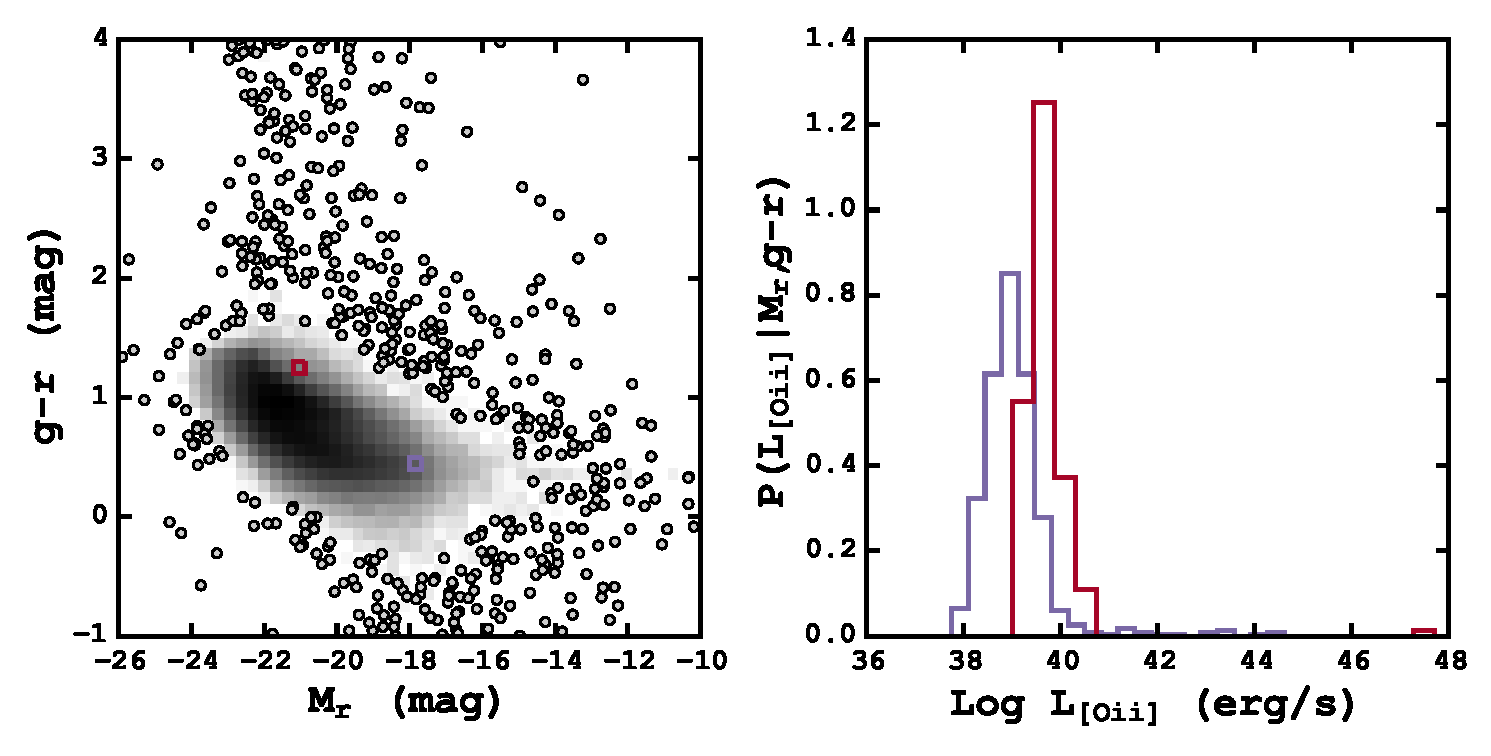
\includegraphics[width=\textwidth]{oii_sdss.pdf} 
	\caption{\textit{Left}: CMD of 503113 $z<0.2$ galaxies take from the SDSS DR12 where the shading scales with the density of points. The two boxes show regions containing potential catalog galaxies. \textit{Right}: Probability histograms of the Log [\ion{O}{2}] luminosity for the SDSS galaxies located in the two highlighted regions on the right. New [\ion{O}{ii}] luminosity (and subsequently fluxes) are assigned to catalog galaxies from slice sampling the probability histogram.} \label{fig:oii sdss} 
\end{figure*}

The buzzard ``truth'' catalog does not provide [\ion{O}{ii}] luminosities so we must assign them empirically. We use 503113 galaxies from the SDSS Data Release 12 \citep{Alam2015} from $z = 0.05 - 0.2$, which are selected with no redshift warning, and place each galaxy on a color-magnitude diagram (CMD) of $M_r$ and $g-r$, see Figure~\ref{fig:oii sdss}.

To assign an [\ion{O}{ii}] luminosity to each galaxy in our catalog we place the catalog galaxies on the same CMD and select all SDSS galaxies in a small 2D ($M_r$, $g-r$) bin around the galaxy. We extract all of the SDSS galaxies inside that bin and create a histogram of their [\ion{O}{ii}] luminosities. Using a slice sampling technique \citep{Neal1997} we assign the catalog galaxy an [\ion{O}{ii}] luminosity based on the distribution of SDSS galaxies extracted. For catalog galaxies which are placed on the CMD near no, or very few ($1\leq n<10$) galaxies we assign it zero [\ion{O}{ii}] luminosity or the mean luminosity, respectively.

The right panel of Figure~\ref{fig:oii sdss} shows the CMD of all SDSS galaxies. Two potential catalog galaxies are also placed on the CMD ($M_r, g-r = -17.7,~0.49$ and $M_r, g-r = -21.4,~1.24$) and indicated by two colored boxes. The histograms show in the Figure's left panel shows the probability density histograms of the Log [\ion{O}{ii}] luminosity for the SDSS galaxies in the 2D bin. We sample the distribution and assign each catalog galaxy an [\ion{O}{ii}] luminosity which is then converted into a flux.

\subsection{Mock Observations}\label{sec:observations}
\editorial{Not sure this does a good enough job talking about the two different observations.}
Tentatively slated to start in the fall of 2015, HETDEX will perform blind spectroscopy (R $\sim$ 750 in $3500 - 5500~\AAA$) over two fields along the celestial equator. The 300 \degsq, Spring field and 120 \degsq, Fall field will have no preselected targets. Using VIRUS on the 10-m Hobby-Eberly Telescope (HET; \citealt{Ramsey1998}) the completed survey is expected to have an overall fill-factor of 1/4.5, meaning that the entire area could be covered with 4.5 dithers of the entire survey. 

The spectral coverage allows for the detection of [\ion{O}{ii}] ($\lambda\lambda 3727-3729~\AAA$ doublet) emitters to $z\sim 0.5$ and Ca H ($\lambda 3968.5~\AAA$) and K ($\lambda 3933.7~\AAA$) absorption features to $z\sim 0.4$. HETDEX is expected to detect sources with continuum brighter than 22 mag in \sdssg, and emission line strengths above $3.5\times10^{-17}$ \ergscm. So we ``observe'' $z<0.4$ galaxies which meet either the emission line or the magnitude limit. Galaxies $0.4<z<0.5$ are only observed if their emission line strength is sufficient.   

\begin{figure} 
	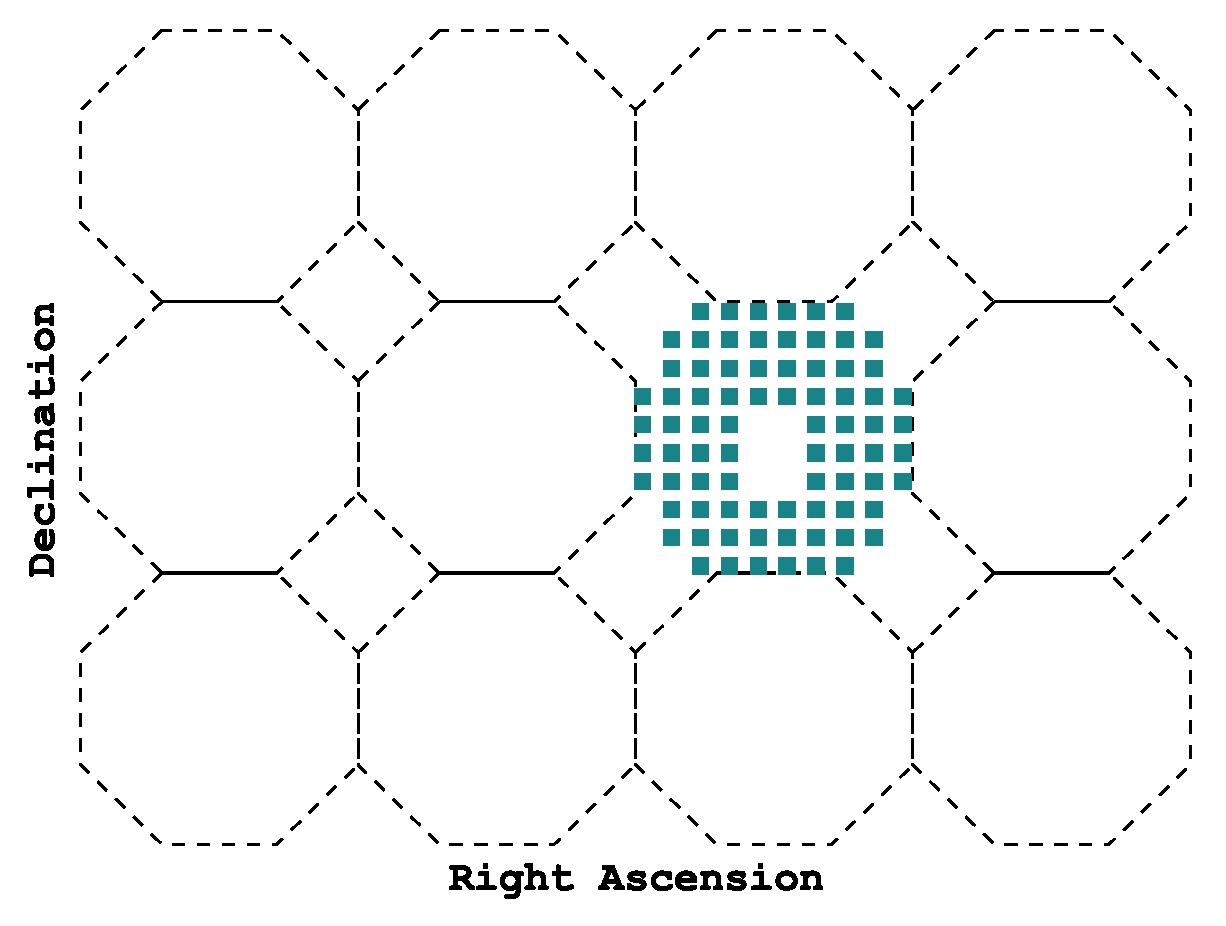
\includegraphics[width=0.49\textwidth]{f01.pdf} 
	\caption{Representative observation tiling scheme for the HETDEX $16'$ pointings. Each colored square is a single VIRUS IFU and the dashed octagons approximate the size of a single observation. See the text for more details.} \label{fig:ifu layout} 
\end{figure}

In this work we consider two separate observation cases. The first are targeted observations where we select each galaxy cluster and ``observe'' each galaxy within $8'$ of the center. The second is a survey case where observations which are blind to the positions of the clusters are conducted. In both cases, our ``observations'' consist of placing masks down onto the buzzard ``truth'' catalogs and selecting all, $z< 0.5$ also meeting sensitivity limits, galaxies which lie underneath. Each mask is created to accurately reproduce the HETDEX IFU pattern, see Figure~\ref{fig:ifu layout}. The pattern consists of 78 IFUs, which are comprised of 448 optical fibers subtending a $50'' \times 50''$ region on the sky \citep{Kelz2014}. The inter-IFU spacing is also $50''$ spanning a total area of $16'\times 16'$ on the sky. 

The individual IFUs have a fill-factor of 1/3, which will be completely filled with three dithers of the telescope at each pointing. This means that when selecting galaxies from the buzzard catalog we assume an observation for all galaxies laying within a colored, IFU square in Figure~\ref{fig:ifu layout}. Galaxies which lie between the IFUs are missed, as well as the galaxies which lie between the pointings, as there is no overlap between one pointing and the next.

\section{Cluster Membership}
In the following sections we assume that the on sky positions and redshifts of the galaxy clusters are already known. In reality, galaxy over densities will be detected from imaging surveys \citeeg{Rykoff2014} or through techniques to identify structure in the RA, DEC, z point data (\eg, DBSCAN; \citealt{Ester1996}).

While the galaxy cluster center may be well known, the constituent galaxies will not. The identification of member galaxies from photometric data \citeeg{Rozo2014} is promising, however, with spectroscopic information on all galaxies, we choose to utilize the full 3D parameter space. \editorial{Not very happy about that sentence}.

We employ the ``shifting gapped" method of \cite{Fadda1996} as outlined in \cite{Owers2011}, which combines both the positional and velocity information. After an initial cut of $cz_c \pm 10,000$ \kms, the galaxies are binned in $0.4h^{-1}$ Mpc or larger enough bins to contain at least 10 (arbitrarily chosen) galaxies. Galaxies farther than 3 Mpc from the cluster center are also rejected. Once binned, the galaxies are sorted by their line-of-sight velocity (LOSV; see Section~\ref{sec:LOSVD}). Any galaxy with a LOSV greater than 1000 \kms of a neighboring galaxy is rejected as an interloper. The procedure repeats until the number of galaxies stabilizes in the bin.

\editorial{This is taken from the other paper, and needs to be tweaked to make fit better into this framework. I think what we'll do is center a 100'' box on all of the clusters and then try to recover the galaxies. How many will we get, how many are wrong, and can we do better with a different algorithm?}

\section{Recovery of Parameters}\label{sec:recovery}
 In the following sections, we outline the methods we use to derive the dynamical properties of the galaxy clusters in our sample. This is not meant to be an exhaustive study of the different methods used to recover these parameters. The following is, in many cases, a subset of the available methods to derive any single parameter. The specific choice of method may improve or diminish the accuracy of the recovered parameter, but the methods chosen were to facilitate comparison with observational studies.  

\subsection{Cluster Redshift}
The accurate determination of the cluster redshift ($z_c$) is crucial to the reliability of all following measurements. An incorrect cluster redshift introduces errors into the measured line of sight velocity (LOSV) and corresponding dispersion, which, in turn, contributes to errors associated with dynamical mass and radius. 

In simple terms, the cluster redshift is the  mean of the redshifts of all galaxies associated with the cluster. However, because the standard mean can be quite sensitive to outliers or otherwise contaminated data, we require a more resistant statistic, and turn to the biweight location estimator \citep{Beers1990} which provides improved performance. 

\subsection{Line of Sight Velocity Dispersion}\label{sec:LOSVD}
We first calculate the line of sight velocity (LOSV) to each galaxy, where
\begin{equation}
	LOSV = c\frac{z - z_c}{1+z_c}
\end{equation}
and $c$ is the speed of light in \kms, $z$ is the redshift of the individual galaxy, and $z_c$ is the overall cluster redshift described in the previous section.

The unbiased estimation of a standard deviation (a measure of statistical dispersion) from these LOSVs is a technically involved problem. At first, we require that our estimator be unbiased in that the dispersion estimation is equal to the true dispersion regardless of the number of points sampled, although, in practice this rarely occurs. The most commonly used estimate is the corrected sample standard deviation, given by:
\begin{equation}
	s = \sqrt{\frac{1}{n-1} \sum_{i=1}^n (x_i - \bar{x})^2}
\end{equation}
with $\{x_1, x_2, ..., x_n\}$ being the random sample and $\bar{x}$ the sample mean. The corrected sample standard deviation has the advantage in that it is unbiased (as opposed to the population standard deviation which is biased), but the removal of bias relies on knowing \textit{a priori} the underlying distribution from which the sample is drawn. An estimator which correctly estimates a standard deviation for a sample drawn from a wide range of distributions and is not adversely effected by outliers is said to be robust. An estimator which correctly identifies the standard deviation, even when a number of points are replaced by different values is said to be resistant.

In our situation, a resistant estimator becomes critical as it minimizes the effect of outliers which the inclusion of non-cluster members have on the measured dispersion. \cite{Beers1990} present both a robust and resistant estimation of scale (yet another term for statistical dispersion) called the biweight scale estimator, which has been widely accepted by the community (\eg, \citealt{Milvang-Jensen2008, Owers2011, Murphy2011} and many others). It is given by 
\begin{equation}
	\sigma_{BI} = \sqrt{ N_{members} \frac{ \sum_{|u_i|<1} (1-u_i^2)^4 (v_i - \bar{v})^2} {D} }
\end{equation}
with $v_i$, the proper velocities, $\bar{v}$, the average of the proper velocities,
\begin{equation}
	D = \sum_{|u_i|<1} (1-u_i^2)(1-5u_i^2)
\end{equation}
with $u_i$ being the biweight weighting and defined as:
\begin{equation}
	u_i = \frac{v_i - \bar{v}}{9 {\rm MAD}(v_i)}
\end{equation}
where MAD is the median absolute deviation. \cite{Ruel2014} note, however, that the biweight scale estimator is biased and suggest a correction of $1/(D-1)$ to $\sigma_{BI}$ referring to it as the biweight sample variance. We adopt this method for clusters with at least 15 members. For clusters with fewer than 15 members, we adopt the gapper scale estimator \citep{Beers1990} which is shown to accurately recover the dispersion for as few as 5 member galaxies \citep{Hou2009}.

There are several situations which can adversely effect the quality of our velocity dispersion measurement. The first is due to the nature of our observations. Because the HETDEX survey has a 1/4.5 fill factor (see Section~\ref{sec:observations}), there will be many situations where we will not have full spectroscopic information for a cluster. Some clusters could also have intrinsic velocity distributions where the observations of only a few members could result in a LOSVD which differs by large percent. This gives rise to clusters along a fixed mass having a large range of possible LOSVDs. \cite{Saro2013} find this effect to be most pronounced for clusters with fewer than 30 members, and \cite{Ruel2014} show the effect is a net increase in scatter of about 5\% compared to clusters with greater than 30 members. \editorial{This section was adapted, pretty heavily from Ruel2014. Is that cool?}

A second effect, unique to works such as this, is the difference between the LOSVD computed between dark matter halos and the galaxies that occupy them, the so-called velocity bias \citeeg{Evrard2008, White2010}. This effect is assumed to be small ($\sim5\%$) and for this work we assume there is no bias, or that the galaxies perfectly trace the velocity distribution.

\subsection{Dynamical Mass}\label{sec:mass}
Recently, the relationship between the LOSVD and dynamical mass has been the focus of several studies \citeeg{Evrard2008, Saro2013, Sifon2013, VanderBurg2014}, and a best fitting relationship for the mass enclosed by $r_{200c}$ of the form
\begin{equation}
	M_{200c} = \frac{10^{15}}{h(z)} \bigg{(}\frac{\sigma_{1D}}{A_{1D}} \bigg{)}^{1/\alpha} \Msol
\end{equation}
with $A_{1D} =$ 1040-1140 \kms\ (\citealt{Munari2013}; referred to as $\sigma_{15}$ in \citealt{Evrard2008} and other works), $\alpha = 1/3$, $h(z) = H(z)/100$, and $\sigma_{1D}$ is the LOSVD of the velocity tracers (dark matter particles, subhalos or galaxies).

The choice $A_{1D}$ and $\alpha$ varies between studies \citeeg{Munari2013, VanderBurg2014} and should be calibrated on a individual basis. To do this, we randomly select 47494, $z<0.5$ clusters composed of 36000 $10^{13}$, 6000 $10^{14}$ and two $10^{15}~\Msol$ halos. We perform a linear fit to the $\sigma_{1D}-M_{200}$ values allowing both $A_{1D}$ and $\alpha$ to vary. We find best fitting parameters of $A_{1D} = 1117.9~\kms$ and $\alpha = 0.3297$, both of which are very near the values from \cite{Evrard2008} of $A_{1D} = 1082.9 \pm 4.0~\kms$ and $\alpha = 0.3361$. Therefore, we chose to adopt the parameters from \cite{Evrard2008} to better facilitate with other simulations \citeeg{Old2014}, and observational studies \citeeg{Brodwin2010}.

\subsection{Radial Extent}
We define the radius of a galaxy cluster as
\begin{equation}
	r_{200c} = \bigg{[} \frac{3}{4\pi} \frac{M_{200}}{200\rho_c} \bigg{]}^{1/3}
\end{equation}
where $\rho_c$ is critical density of the universe and defined as $3H^2/8\pi G$.

\section{RESULTS}\label{sec:results}
The results of this work come in two broad sections. The accuracy of which we determine each cluster's LOSVD and dynamical mass, and the probability given a determined mass it is the correct mass. We test two different observation strategies with ideal and realistic information about the membership of the observed galaxies. Ideal information is knowing the exact membership of the galaxies, and realistic information relies on methods to determine the membership. \editorial{The results of this section a shown in Figures XXX and Figures XXX for the LOSVD and masses respectively.}

\subsection{Targeted, Ideal Observations}
\subsection{Targeted, Realistic Observations}
\subsection{Blind, Ideal Observations}
\subsection{Blind, Realistic Observations}
We compare the calculated cluster redshifts to the true redshift ($z_{c,true}$) for 114903 galaxies comprising 1379 unique halos, and we find a RMS$[\Delta z/(1+z_{c,true})]= 4\times 10^{-4}$ where $\Delta z = z_{c,true} - z_{c}$. \editorial{The RMS using just the regular mean is 3.8e-4 which is only slightly better than the biweight. I don't think that will be the case when we get more complicated things.}

\begin{figure*} 
	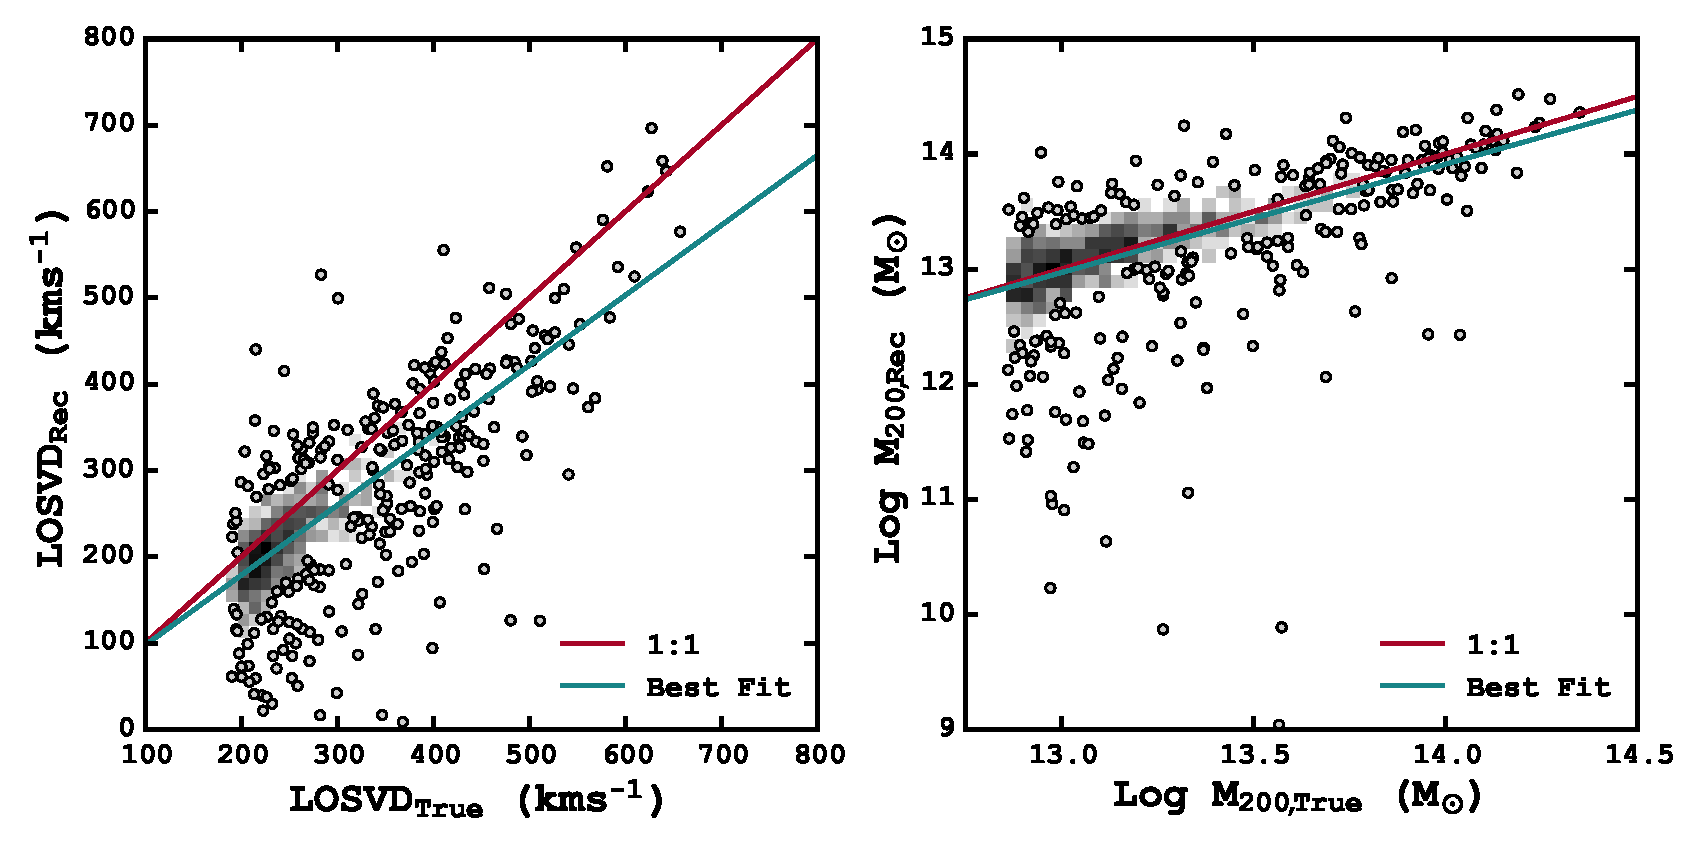
\includegraphics[width=\textwidth]{fullKnowledge.pdf} 
	\caption{Intrinsic cluster properties versus the recovered cluster properties for 16758 unique halos comprised of 657916 individual galaxies. The left panel shows the line of sight velocity dispersion (LOSVD) and the right panel shows the recovered halo mass. In both panels, the red line shows the 1:1 relation and the teal line shows the best fit to data.} 
	\label{fig:full} 
\end{figure*}

\begin{figure*} 
	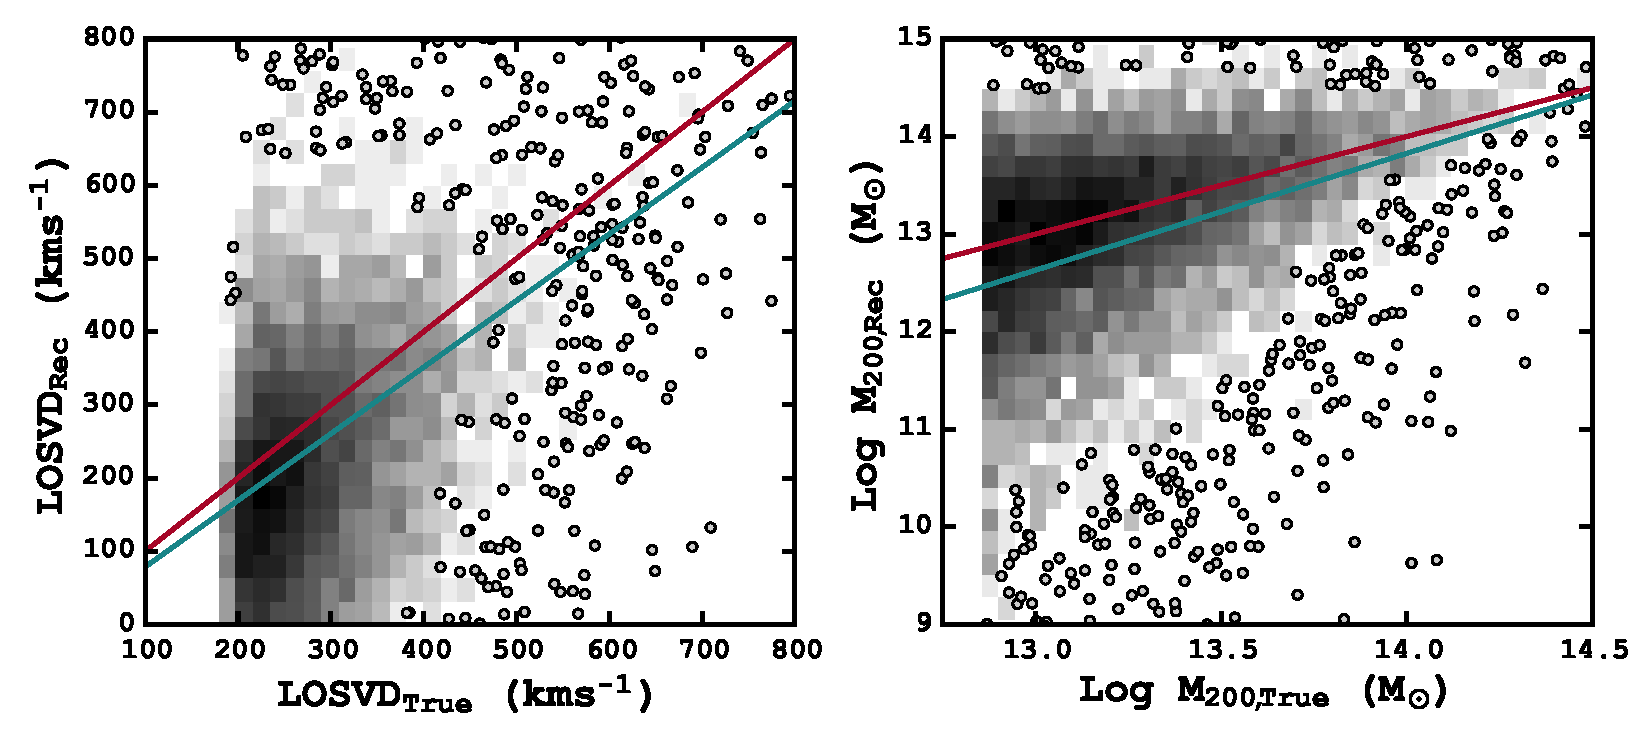
\includegraphics[width=\textwidth]{hetdexDepth.pdf} 
	\caption{HETDEX DEPTH! Intrinsic cluster properties versus the recovered cluster properties for 14239 unique halos comprised of 87754 individual galaxies. The left panel shows the line of sight velocity dispersion (LOSVD) and the right panel shows the recovered halo mass. In both panels, the red line shows the 1:1 relation and the teal line shows the best fit to data.} 
	\label{fig:hetdexDepth} 
\end{figure*}
Lorem ipsum dolor sit amet, consectetur adipisicing elit, sed do eiusmod tempor incididunt ut labore et dolore magna aliqua. Ut enim ad minim veniam, quis nostrud exercitation ullamco laboris nisi ut aliquip ex ea commodo consequat. Duis aute irure dolor in reprehenderit in voluptate velit esse cillum dolore eu fugiat nulla pariatur. Excepteur sint occaecat cupidatat non proident, sunt in culpa qui officia deserunt mollit anim id est laborum.


\section{SUMMARY}
Lorem ipsum dolor sit amet, consectetur adipisicing elit, sed do eiusmod tempor incididunt ut labore et dolore magna aliqua. Ut enim ad minim veniam, quis nostrud exercitation ullamco laboris nisi ut aliquip ex ea commodo consequat. Duis aute irure dolor in reprehenderit in voluptate velit esse cillum dolore eu fugiat nulla pariatur. Excepteur sint occaecat cupidatat non proident, sunt in culpa qui officia deserunt mollit anim id est laborum.

\acknowledgments 
The authors also wish to thank the anonymous referee whose comments and suggestions significantly improved both the quality and clarity of this work. This research made use of This research made use of \textsc{APLpy}, an open-source plotting package for Python hosted at http://aplpy.github.com; the \textsc{IPython} package \citep{Perez2007}; \textsc{matplotlib}, a Python library for publication quality graphics \citep{Hunter2007}. Funding for the SDSS and SDSS-II has been provided by the Alfred P. Sloan Foundation, the Participating Institutions, the National Science Foundation, the U.S. Department of Energy, the National Aeronautics and Space Administration, the Japanese Monbukagakusho, the Max Planck Society, and the Higher Education Funding Council for England. The SDSS Web Site is http://www.sdss.org/. The SDSS is managed by the Astrophysical Research Consortium for the Participating Institutions.

\bibliography{master}

\end{document}

% \section{Evidence of Substructure}
% Like the recovery of dynamical parameters discussed in the previous section, the choice of method to investigate the dynamical state of galaxy clusters is heavily debated. Perhaps the most widely used metric is the Dressler-Shectman (DS) test \citep{Dressler1988}, and is not without criticism \citeeg{White2010}. New methods such as the Caustic Method (\citealt{Yu2015}, and the references therein) offer promise to shed further light on this difficult problem.
%
% \subsection{From VD profiles}
% We utilize the modality \citep{Oliva-Altamirano2014} which describes the Gaussianity of a LOSV distribution in a galaxy cluster. For clusters with Gaussian distributed LOSVs, the modality is close to 1/3. It is defined as $(1+\mathrm{skewness}^2)/(3+\mathrm{kurtosis}^2)$. \editorial{Do I need to describe what the skewness and kurtosis is?}
%
% \subsection{Dominance}
% \editorial{This is taken pretty directly from the GAMA paper. Will need to be edited to fit.}
% The dominance is defined as the luminosity gap between the brightest and the second brightest galaxy in a cluster ($\Delta m_{1, 2}$). The amplitude of the luminosity gap between the BGG/BCG and the second brightest galaxy in the halo, is expected to be a function of both the formation epoch and the recent infall history of the halo. A small magnitude gap ($\Delta m_{1, 2} < 1$) indicates a recent halo merger, and larger gaps ($\Delta m_{1, 2} > 1$), common in fossil groups, is perhaps indicative of a cluster or groups that has not undergone a recent merger.
%
% \subsection{Dressler-Schectman Test}
% We leverage the large spectroscopic dataset to study the structural properties of the clusters. \cite{Pinkney1996} determine, from a comparison of five different methods that the DS test is the most sensitive to the presence of substructure.
%
% The DS test, which combines the spatial positions and velocities of the galaxies, provides a method to locate substructure by identifying groups of galaxies which differ significantly from the cluster velocity distribution. Galaxy subsets are selected from a cluster of $n_{members}$ and each constituent galaxy deviation is calculated according to
% \begin{equation}
% 	\delta_i^2 = \frac{N_{local}+1}{\sigma^2}\bigg{[}(\bar{v}_{local,i} - \bar{v})^2 + (\sigma_{local,i} - \sigma)^2\bigg{]}^2
% \end{equation}
% where $\bar{v}_{local}$ and $\sigma_{local}$ are the mean velocity and velocity dispersion for a subset of $N_{local}$ galaxies and $\bar{v}$ and $\sigma$ are the entire cluster's mean velocity and velocity dispersion. The choice of $N_{local}$ is left to the user. Originally, \cite{Dressler1988} choose $N_{local}=10$, however \cite{Bird1994} points out that using a fixed value for $N_{local}$ reduces the sensitivity to substructure. We follow \cite{Bird1994} in choosing $N_{local} = \sqrt n_{members}$. \editorial{doesn't talk about the nearest neighbors which is what we are using.}
%
% The DS statistic is the $\Delta$-value given by,
% \begin{equation}
% 	\Delta = \sum^{n_{members}}_i \delta_i
% \end{equation}
% where a system is considered to contain substructure if $\Delta/n_{members} > 1$ \citep{Dressler1988}. A second method, described in \cite{Hou2012}, uses probabilities (P-values) rather than a threshold for the identification of substructure. P-values are computed by comparing the observed $\Delta$-value and the $Delta$-value after the velocities (but not positions) have been shuffled through a series of Monte Carlo runs. The probability of the existence of substructure becomes
% \begin{equation}
% 	P = \sum (\Delta_{shuffled} > \Delta_{Observed}) / n_{shuffle}
% \end{equation}
% where $n_{shuffle}$ is the number of shufflings used. \editorial{This sounds a whole lot like the description given in Hou2012. Make sure that we aren't copying anything word for word. That'd be bad.}
%
% In practice, we use locate the nearest neighbors using an unsupervised k-nearest neighbor algorithm as implemented in Scikit-Learn \citep{Pedregosa2012}.
